\chapter{THE ALGORITHM}
\label{ch:Algorithm}
In this chapter we explain the algorithm we came up with to open a string-envelope. The analysis of this algorithm is based on \cite{cormen2009introduction}. We start by showing the initial configuration of the robot, then we explain the algorithm by showing the flowchart followed by the pseudocode and we finish by showing some examples. The output is that the robot opens the envelope that has been previously tied in an arbitrary manner. 

\section{Initial configuration}
In this section, we show the initial configuration of all the elements and the preconditions we need for the algorithm to work correctly.

The initial configuration is shown in Figure~\ref{fig:configuration} below.
\begin{figure}[h!]
	\centering
	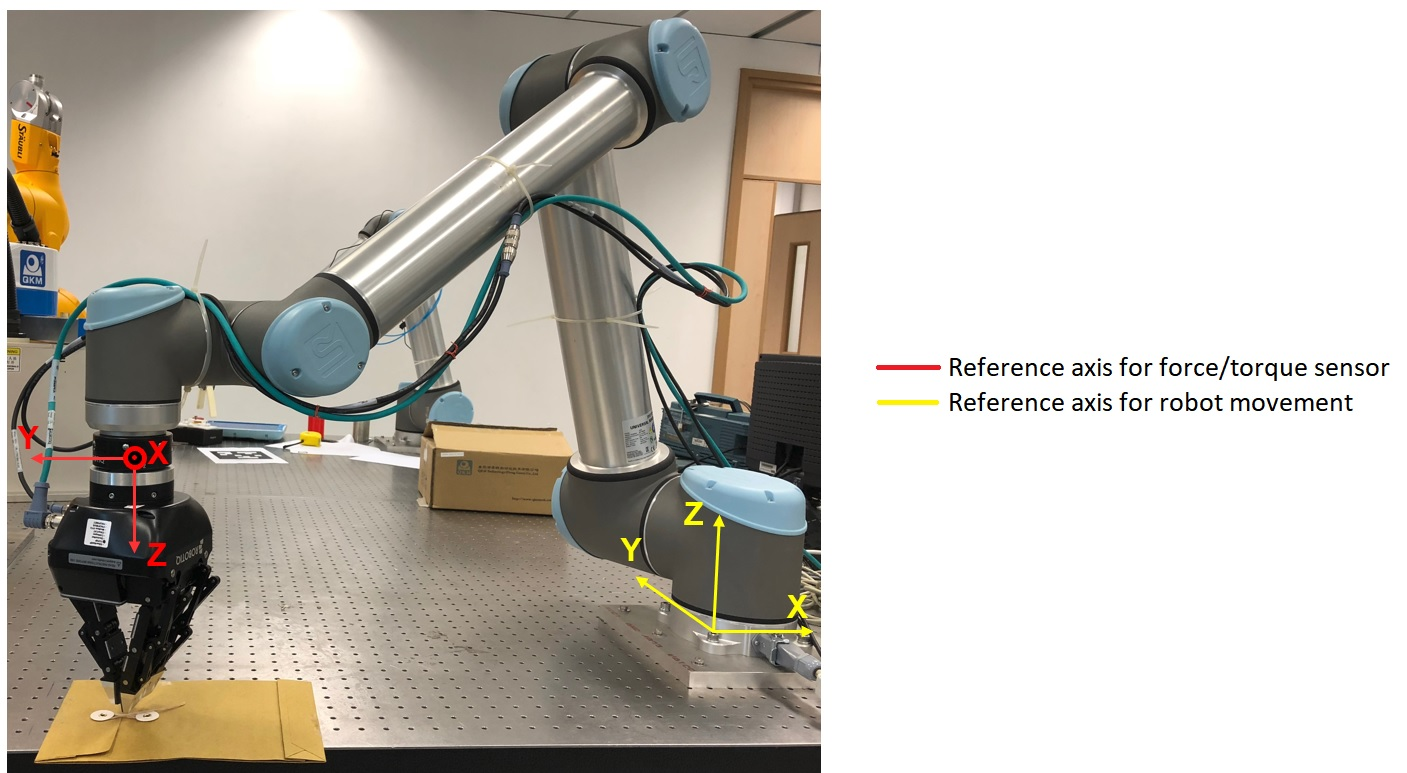
\includegraphics[height=86mm]{chapters/figures/algorithm/configuration.jpg}
	\caption{Initial configuration of the robot and all the elments.}
	\label{fig:configuration}
\end{figure}

The red axis represents the reference for the wrist force-torque sensor and the yellow axis represents the reference for the robot movement.

The preconditions for the algorithm to work are:
\begin{itemize}
 \item The robot is already grasping the string in the middle between the two pivots.
 \item $r_{p}$: Pivots' radius.
 \item $d$: Distance between pivots.
 \item $k$: Threshold value from which the torque sensor reading is considered relevant.
\end{itemize}

We call Pivot 1 to the pivot that is attached to the flap of the envelope and Pivot 2 to the other one. We will use the abbreviation P1 for Pivot 1 and P2 for Pivot 2.

\section{Algorithm}
In this section, we show the flowchart, the pseudocode of the algorithm and some examples to explain how this one works.

\subsection{Flowchart}
The flowchart is shown in Figure~\ref{fig:flowchart}.

% Define block styles
\tikzstyle{decision} = [diamond, aspect=3, draw, fill=blue!20, 
text width=10em, text badly centered, node distance=3cm, inner sep=0pt]
\tikzstyle{block} = [rectangle, draw, fill=blue!20, 
text width=12em, text centered, rounded corners, minimum height=2em]
\tikzstyle{line} = [draw, -latex']
%\tikzstyle{cloud} = [draw, ellipse,fill=red!20, node distance=3cm, minimum height=2em]
\begin{figure}[h]
\begin{center}
\begin{tikzpicture}[node distance = 2.5cm, auto]
% Place nodes
\node [block] (init) {Start};
\node [block, below of=init, node distance=1.8cm] (move) {Move $2 \cdot r_{p}$ in perpendicular to pivots' joining axis};
\node [block, left of=move, node distance=5.5cm] (return) {Return to initial pose};
\node [decision, below of=move, node distance=2.2cm] (evaluate) {$|M_{x}| \geq |k|$ and $|M_{y}| \geq |k|$?};
\node [block, below of=evaluate, node distance=2.6cm] (decide) {Turn 360$\,^{\circ}$ about the right pivot in the right direction};
\node [decision, below of=decide, node distance=2.2cm] (evaluate1) {$|M_{y}| \geq |k|$?};
\node [block, below of=evaluate1,  node distance=2.4cm] (move1) {Move $2 \cdot r_{p}$ in perpendicular and outwards pivots joining axis};
\node [block, left of=move1, node distance=5.5cm] (same_pivot) {Turn 360$\,^{\circ}$ about the same pivot in the same direction};
\node [decision, below of=move1, node distance=2.4cm] (evaluate2) {$|M_{y}| \geq |k|$?};
\node [block, below of=evaluate2,  node distance=2.5cm] (opsd) {Turn in the same direction about the opposite pivot};
\node [block, left of=opsd, node distance=5.5cm] (opod) {Turn in the opposite direction about the opposite pivot};
\node [decision, below of=opsd, node distance=2.5cm] (evaluate3) {Gripper turning about P1?};
\node [block, right of=evaluate3, text width=9em, node distance=6cm] (continue) {Keep going until turn complete};
\node [decision, below of=evaluate3, node distance=2.8cm] (evaluate4) {$|M_{x}| \geq |k|$ or $|M_{y}| \geq |k|$?};
\node [block, left of=evaluate4, text width=6em, node distance=6cm] (stop) {Stop};

% Draw edges
\path [line] (init) -- (move);
\path [line] (move) -- (evaluate);
\path [line] (evaluate) -| node [near start] {no} (return);
\path [line] (return) |- (move);
\path [line] (evaluate) -- node {yes}(decide);
\path [line] (decide) -- (evaluate1);
\path [line] (evaluate1) -| node [near start] {yes} (same_pivot);
\path [line] (same_pivot) |- (evaluate1);
\path [line] (evaluate1) -- node {no} (move1);
\path [line] (move1) -- (evaluate2);
\path [line] (evaluate2) -| node [near start] {yes} (opod);
%\path [line] (opod) |- (evaluate2);
\path [line] (evaluate2) -- node {no} (opsd);
\path [line] (opod) |- (evaluate3);
\path [line] (opsd) -- (evaluate3);
\path [line] (evaluate3) -- node {no} (continue);
\path [line] (continue) |- (evaluate1);
\path [line] (evaluate3) -- node {yes} (evaluate4);
\path [line] (evaluate4) -| node [near start] {no} (continue);
\path [line] (evaluate4) -- node {yes} (stop);
\end{tikzpicture}
\end{center}
\caption{Flowchart of the algorithm to open a string-envelope.}
\label{fig:flowchart}
\end{figure}
\clearpage

The algorithm starts and the gripper moves $2 \cdot r_{p}$ in perpendicular to pivots' joining axis. If absolute values of torques around x-axis and y-axis are less than absolute value of threshold, the the gripper returns to the initial pose and it moves $2 \cdot r_{p}$ in perpendicular to pivots' joining axis, but in the opposite direction. Otherwise,  if absolute values of torques around x-axis and y-axis are greater than absolute value of threshold, then the gripper turns 360$\,^{\circ}$ about the right pivot in the right direction to untie the string, depending on the sign of torques. 

After one turn, if absolute value of torque around y-axis is greater than absolute value of threshold, then the string is tied about the same pivot and the gripper will turn 360$\,^{\circ}$ about the same pivot in the same direction. Otherwise, the gripper will move $2 \cdot r_{p}$ in perpendicular and outwards pivots' joining axis. There, if absolute value of torque around y-axis is greater than absolute value of threshold, the gripper will turn in the opposite direction about the opposite pivot to untie the string. Otherwise, the gripper will turn in the same direction about the opposite pivot to untie the string.

To know whether the string has completely been untied, it is important to know that the beginning of the string is always attached to P1. So, if the gripper is turning about P1 to try to untie the string and absolute values of torques around x-axis and y-axis increase over absolute value of threshold, then the string is completely untied and the movement stops and the algorithm ends. The fact that torque values increase during the movement about P1 means that the string has completely been untied because its length won't increase anymore while the gripper is "openning" the movement to try to untie the string.

\subsection{Pseudocode}
The pseudocode is presented as a procedure called \textbf{UNTIE-STRING} and it is shown below.
\begin{algorithm}
	\caption{UNTIE-STRING}\label{euclid}
	\begin{algorithmic}[1]
%		\Procedure{MyProcedure}{}
		\State $\textit{turn} \gets \text{0}$
		\State $[\textit{p}, \textit{c}] \gets \textbf{evaluateTorques}$
		\State Turn about \textit{p} in direction \textit{c}
		\While {True}
		\State $[\textit{p}, \textit{c}] \gets \textbf{evaluateTorques}$
		\State Turn about \textit{p} in direction \textit{c}
		\If {$\textit{p} = \textit{P1}$}
		\State Store $M_{x}$, $M_{y}$ during the movement
		\If {$|M_{x}| > \textit{k}$ or $|M_{y}| > \textit{k}$}
		\State \textbf{break}
		\Else 
		\State keep going
		\EndIf
		\EndIf
		\EndWhile
	\end{algorithmic}
\end{algorithm}

The algorithm can be divided in two parts. First part goes from line 1 to 3 and second part goes from line 4 to 12. 

The first part of the algorithm makes the first turn to start untying the string. There are four possible movements:
\begin{itemize}
	\item Rotate clockwise (CW) about P1.
	\item Rotate counterclockwise (CCW) about P1.
	\item Rotate clockwise about P2.
	\item Rotate counterclockwise about P2.
\end{itemize}

Then, for the second part of the algorithm (\textbf{while} loop), after the first turn, there are only three possible movements:
\begin{itemize}
	\item Rotate about the same pivot in the same direction.
	\item Rotate about the other pivot in the other direction.
	\item Rotate about the other pivot in the same direction.
\end{itemize}

Let's start by explaining how the algorithm makes the first movement (lines 1-3).
In line 1, the variable \textit{turn} is initialized to 0. This variable lets know whether we are in the first turn or after.
In line 2, the function \textbf{evaluateTorques} determines which pivot, \textit{p}, and direction, \textit{c}, to turn in order to untie the string, depending on torque values $M_{x}$ and $M_{y}$. This function is shown and explained later. In line 3, the first turn is executed.

After the first turn, we enter the \textbf{while} loop (lines 4-12). Here, the algorithm makes the rest of the turns and stops when the string has completely been untied. In line 5, again the \textbf{evaluateTorques} function determines the pivot \textit{p} and the direction \textit{c} to untie the string and the movement is executed in line 6. 

For the algorithm to be correct and complete, it has to determine whether the string has completely been untied or not. Once the envelope is opened, the algorithm must finish. 

As explained before, if the gripper is turning about P1 (line 7), then torques $M_{x}$ and $M_{y}$ will be stored during the movement (line 8). If torque values increase, then the movement will stop and the algorithm will finish (lines, 9, 10). 

The pseudocode for the \textbf{evaluateTorques} function is shown below:
\begin{algorithm}
	\caption{evaluateTorques}\label{euclid}
	\begin{algorithmic}[1]
		%		\Procedure{MyProcedure}{}
		\If {$\textit{turn} = 0$}
		\State $[M_{x}, M_{y}] = \textbf{pullString(0, $\pm2 \cdot r_{p}$)}$
		\If {$M_{y} > \textit{k}$ and $M_{x} < \textit{-k}$}
		\State $\textit{p} = \textit{P1}, \textit{c} = \textit{CW}$
		\ElsIf {$M_{y} > \textit{k}$ and $M_{x} > \textit{k}$}
		\State $\textit{p} = \textit{P2}, \textit{c} = \textit{CCW}$
		\ElsIf {$M_{y} < \textit{-k}$ and $M_{x} < \textit{-k}$}
	
		\algstore{myalg}
	\end{algorithmic}
\end{algorithm}

\clearpage
		
\begin{algorithm}
%	\ContinuedFloat
	\caption{evaluateTorques (continued)}
	\begin{algorithmic}
		\algrestore{myalg}
		\State $\textit{p} = \textit{P1}, \textit{c} = \textit{CCW}$	
		\ElsIf {$M_{y} < \textit{-k}$ and $M_{x} > \textit{k}$}
		\State $\textit{p} = \textit{P2}, \textit{c} = \textit{CW}$
		\EndIf
		\State $turn \hspace{0.2cm}+=1$
		\EndIf
		\If {$\textit{turn} > 0$}
		\State Store $M_{x}$, $M_{y}$
		\If {$|M_{y}| > \textit{k}$}
		\State \textit{p} and \textit{c} remain the same as in previous turn
		\Else
		\State $[M_{x}, M_{y}] = \textbf{pullString(0, $\pm2 \cdot r_{p}$)}$
		\If {$|M_{y}| > \textit{k}$}
		\State \textit{p} and \textit{c} are the opposite as in previous turn
		\Else
		\State \textit{p} is the opposite as in previous turn, \textit{c} remains the same
		\EndIf
		\EndIf
		\EndIf
		\Return {p, c}
	\end{algorithmic}
\end{algorithm}

The decision of which pivot and wich direction to turn is made inside the \textbf{evaluateTorques} function. The decision for the first turn is made from line 1 to line 11 and the decision for the rest of the turns is made from line 12 to line 21. 

For the first turn (lines 1-11), the gripper starts moving $2 \cdot r_{p}$ in perpendicular to pivots' joining axis (line 2).

Being on the right side of the pivots:
\begin{itemize}
	\item If $M_{y}$ is greater than $k$ and $M_{x}$ is less than $-k$, then the right movement to untie the string is to turn CW about P1 (lines 3, 4).
	\item If $M_{y}$ and $M_{x}$ are greater than $k$, then the right movement to untie the string is to turn CCW about P2 (lines 5, 6).
\end{itemize}

Being on the left side of the pivots:
\begin{itemize}
	\item If $M_{y}$ and  $M_{x}$ are less than $-k$, then the right movement to untie the string is to turn CCW about P1 (lines 7, 8).
	\item If $M_{y}$ is less than $-k$ and $M_{x}$ is greater than $k$, then the right movement to untie the string is to turn CW about P2 (lines 9, 10).
\end{itemize}

Then, the variable $turn$ is updated (line 11), so we know the first turn has already been made.

To figure out the rest of the turns (lines 12-21), we start by storing $M_{x}$ and $M_{y}$ values at the end of one turn (line 13). Then:

\begin{itemize}
	\item If $|M_{y}|$ is greater than $|k|$, then the gripper has to continue turning in the same direction about the same pivot to untie the string (lines 14, 15).
\end{itemize}

Otherwise, if at the end of one turn, absolute value of torque around y-axis is less than absolute value of threshold, then the string is tied about the other pivot. To know which direction to turn, the gripper will move $2 \cdot r_{p}$ in perpendicular and outwards pivots' joining axis (line 17). Then:
\begin{itemize}
	\item If $|M_{y}|$ is greater than $|k|$, then the right movement to untie the string is the opposite pivot and the opposite direction than in the previous turn (lines 18, 19).
	\item If $|M_{y}|$ is less than $|k|$, then the right movement to untie the string is the opposite pivot and the same direction than in the previous turn (lines 20, 21).
\end{itemize}

This function returns the pivot, \textit{p}, and the direction, {c}, to the main function.

After the first turn, we ignore torque around x-axis value because as the gripper unties the string and goes farther from pivots, the distance between the gripper and the pivots is much greater than the distance between pivots. As at the end of one turn the string is almost perpendicular to pivots' joining axis, torque around x-axis is almost 0 and does not allow to distinguish wich pivot to turn.

The pseudocode for the \textbf{pullString(0, $2 \cdot r_{p}$)} function (lines 2, 17), that consists of moving the gripper $2 \cdot r_{p}$ and storing $M_{x}$ and $M_{y}$, is shown below:
\begin{algorithm}
	\caption{pullString(0, $\pm2 \cdot r_{p}$)}\label{euclid}
	\begin{algorithmic}[1]
		%		\Procedure{MyProcedure}{}
		\If {$turn = 0$}
		\State Move 0 in x, $+2 \cdot r_{p}$ in y
		\If {$|M_{y}| < |k|$}
		\State Return to initial pose
		\State Move 0 in x, $-2 \cdot r_{p}$ in y
		\EndIf
		\Else
		\State Move 0 in x, $2 \cdot r_{p}$ in y outwards pivots' joing axis
		\EndIf
		\Return {$M_{x}, M_{y}$}
	\end{algorithmic}
\end{algorithm}

For the first turn (line 1), the gripper starts moving $+2 \cdot r_{p}$ in y-axis (line 2). If absolute value of torque around y-axis is less than absolute value of threshold, then the gripper returns to the initial pose and moves $-2 \cdot r_{p}$ in y-axis (lines 3-5).

After the first turn (line 6), the gripper moves $2 \cdot r_{p}$ in y-axis outwards pivots' joining axis (line 7). 

This function returns $M_{x}$ and $M_{y}$ values to the \textbf{evaluateTorques} function.

Now, we will show some examples of how the algorithm works.

\subsection{Examples}
For a better understanding of what we explained before, we show here some examples of how the algorithm works to figure out the first turn, the rest of the turns and the end of the movement. 

We start by showing an example of how the algorithm figures out the first turn. Figure~\ref{fig:first_turn} shows the four possible cases for the first turn.
\begin{figure}[h!]
	\centering
	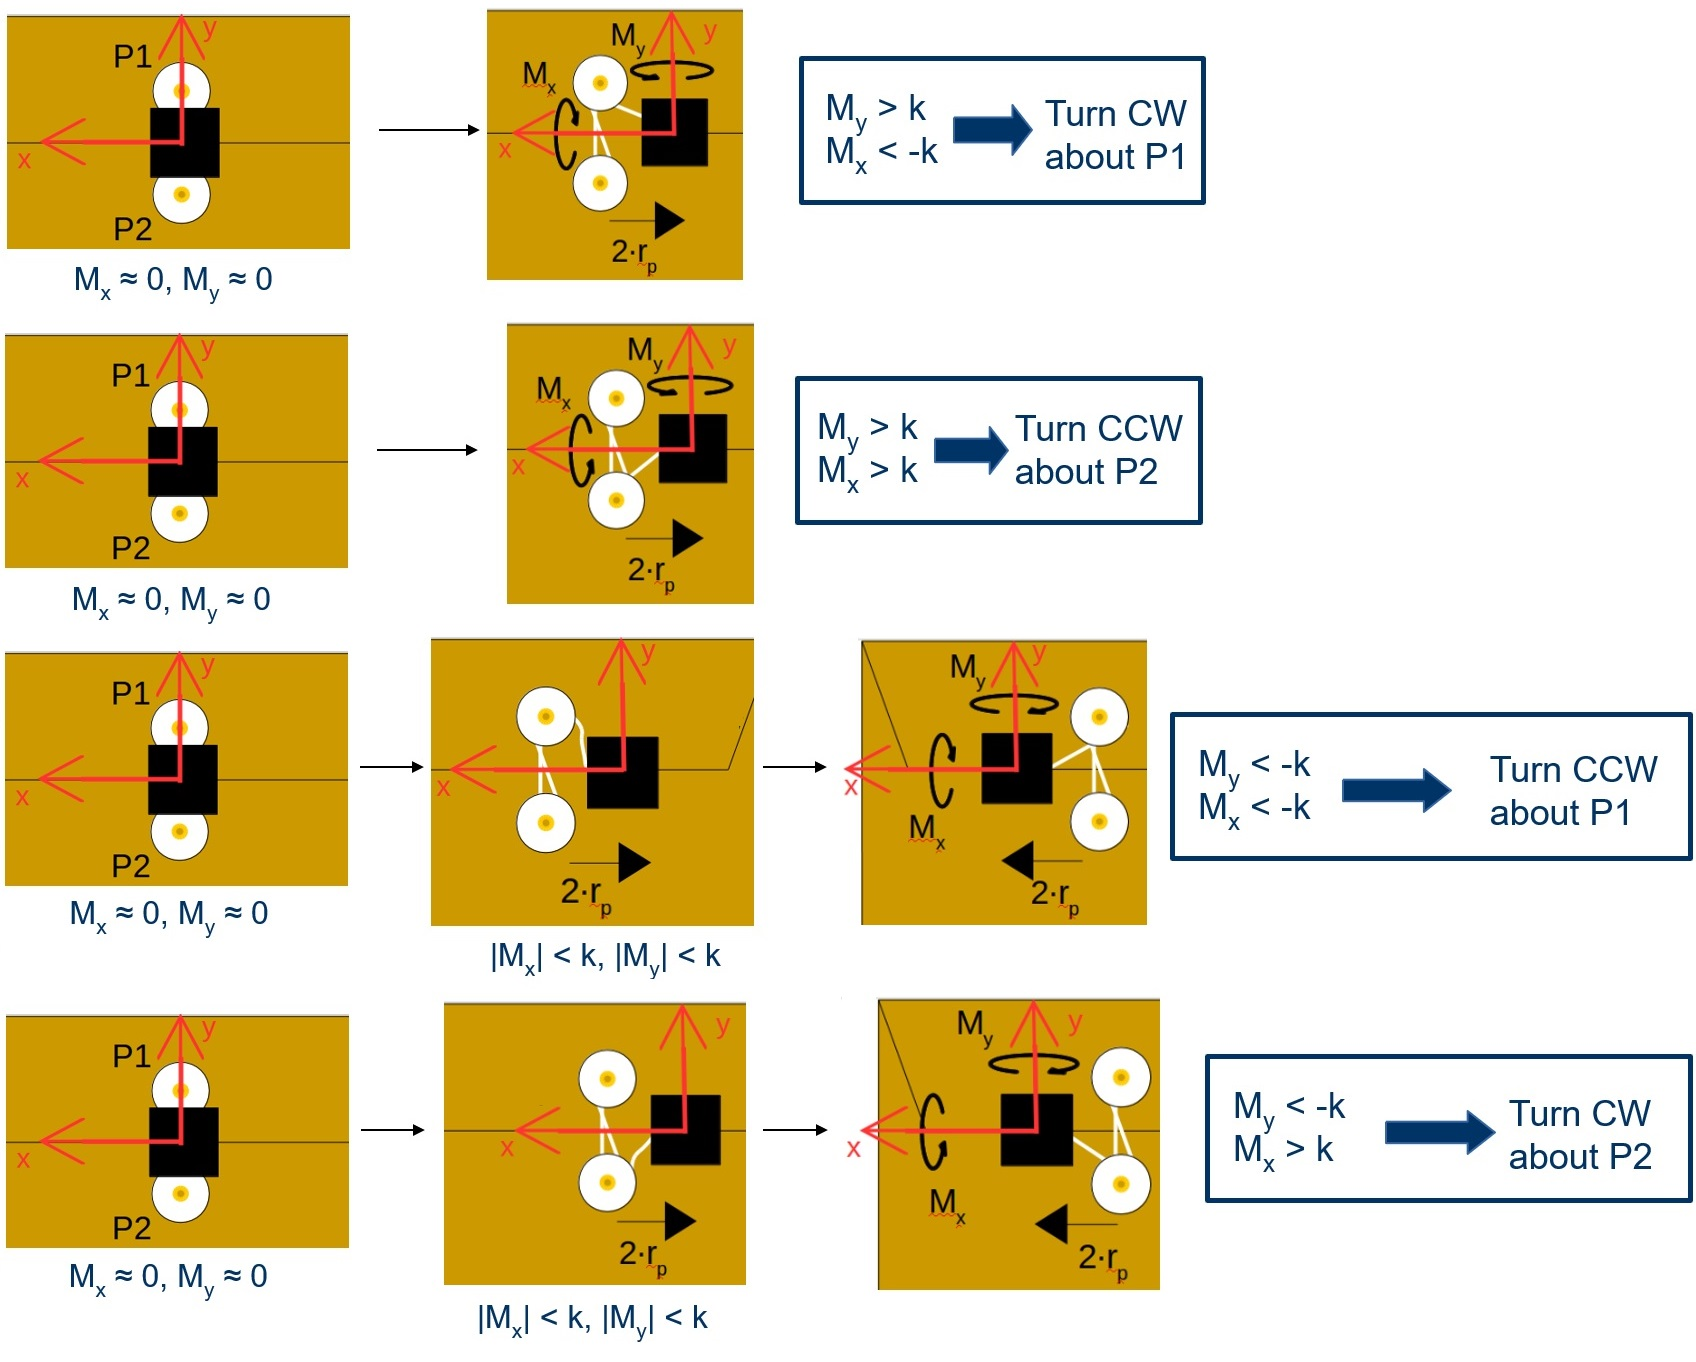
\includegraphics[height=130mm]{chapters/figures/algorithm/first_turn.jpg}
	\caption{Example of how the algorithm figures out the first turn.}
	\label{fig:first_turn}
\end{figure}

Let's tell the first turn was CW about P1, then Figure~\ref{fig:same_pivot} shows what happens after this turn if the string is again tied about the same pivot.
\begin{figure}[h!]
	\centering
	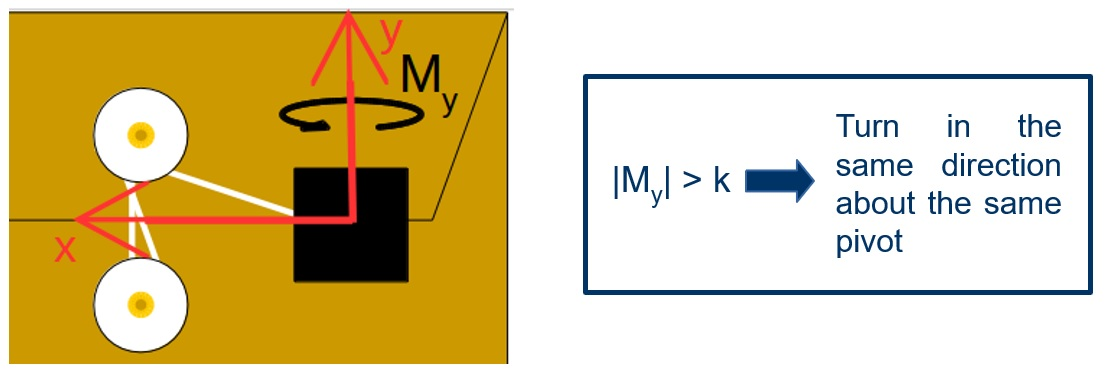
\includegraphics[height=40mm]{chapters/figures/algorithm/samepivot.jpg}
	\caption{Example of the case where the string is tied about the same pivot after one turn.}
	\label{fig:same_pivot}
\end{figure}

Otherwise, if the string is tied about the other pivot after the first turn, Figure~\ref{fig:other_pivot} shows what happens:
\begin{figure}[h!]
	\centering
	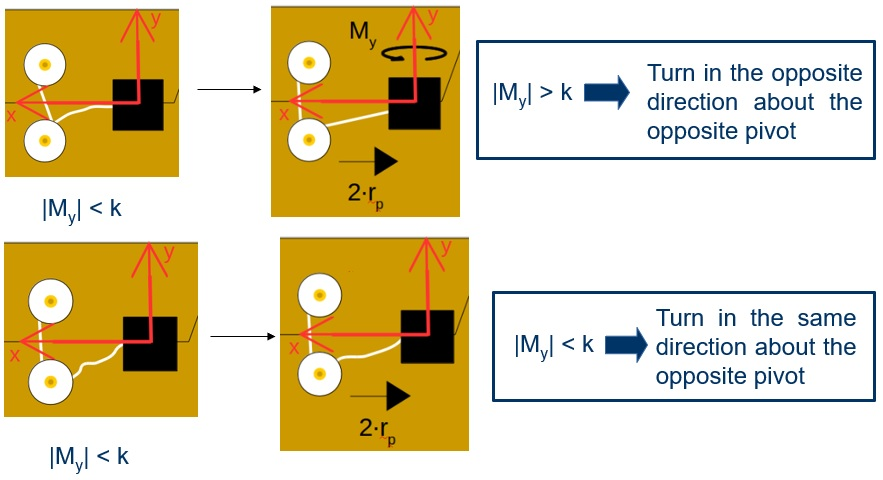
\includegraphics{chapters/figures/algorithm/otherpivot.jpg}
	\caption{Example of the cases where the string is tied about the other pivot after one turn.}
	\label{fig:other_pivot}
\end{figure}

 Finally, Figure~\ref{fig:end} shows how the algorithm figures out the end of the movement.
\begin{figure}[h!]
	\centering
	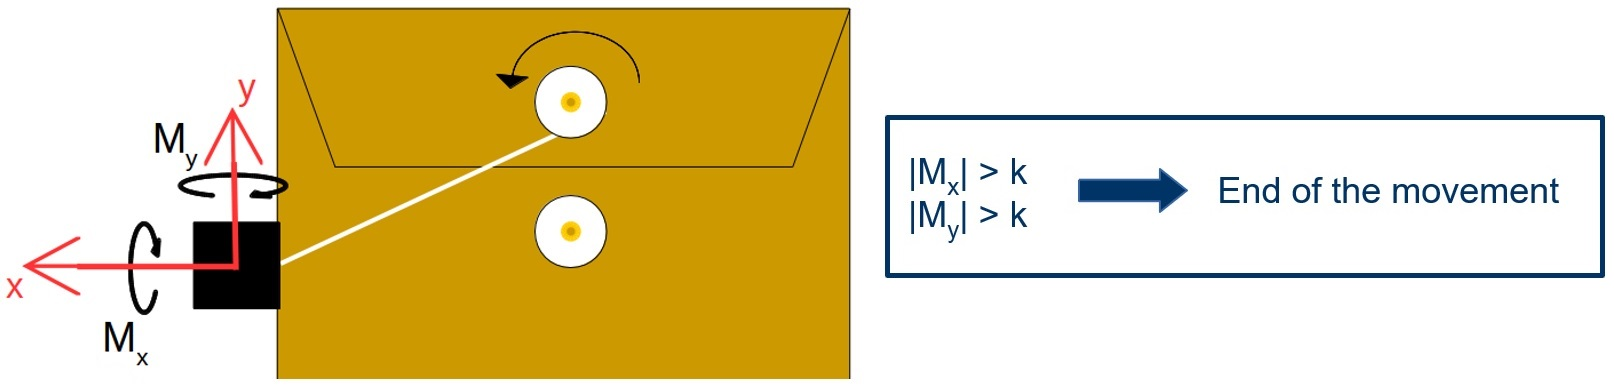
\includegraphics[height=40mm]{chapters/figures/algorithm/end.jpg}
	\caption{Example of the end of the movement.}
	\label{fig:end}
\end{figure}
\clearpage

%The word \textit{\textbf{robot}}\index{Robot} represents a very general concept that is hard to define precisely, since this word can be used to name a great amount of machines. 
%
%The aim of this chapter is to give an approximation to the concept of robot. Thus a brief history of robotics, the two technological roots of robotics, and finally an explanation to basic robotic jergon are presented.
%
%Let's start with a little riddle: which the following examples are robots?
%\begin{itemize}
% \item An automatic camera?
% \item An automatic washing machine?
% \item An automatic dishwasher?
% \item An automatic car (a car with an automatic gearbox)?
% \item A crane\footnote{gr\'ua}?
%\end{itemize}
%
%For some people, some or all of these examples are kinds of robots, for others none of them are. It all depends on what our own idea of what a robot is, and this can vary a lot from person to person.
%The word robot is often related with some kind of machine that has similarities to some part of human (or animal), body.  But this is not always true \ldots
%
%\section{A Little about the History}
%Although in appendix \ref{ch:introduntion} a review is made of remarkable milestones in \textit{\textbf{Robot history}} from the Ancient Greek culture to the present, let's see only the beginning of modern robotics. 
%
%The word robot was used for the first time in 1920 in a play entitled \textit{\textbf{R.U.R.}}\index{R.U.R} (\textit{\textbf{Rosum's Universal Robots}}\index{Rosum's Universal Robots}). This play was written by \textit{\textbf{Karel Capek}}\index{Karel Capek}, a Czech playwright. In the original Czeck, \textit{\textbf{Robota}}\index{Robota} means forced servitude. The name Rossum is an allusion to the Czech word rozum, which means reason, intellect. After the production of R.U.R. opened, the word robot displaced older words such as automaton or android in most languages. R.U.R stands for ''Rosumovi Um\v{e}l\'i Roboti'' (Mr. Reasson's Artificial Robots) and when the play was first put on in English-speaking countries, this title was translated from the Czech as ''Rossum's Universal Robots'' in order to fit the initials R.U.R (Figure~\ref{fig:rur}).
%
%\begin{figure}[htbp]
% \centering
% \includegraphics{chapters/figures/1_01_rur.jpg}
% \caption{A representation of a Rossum's Universal Robot.}
% \label{fig:rur}
%\end{figure}
% 
%In Capek's play, robots were human-like (humanoid) machines that were created by Rossum and his son to become servants of real human beings. But robots end up not accepting this role and rebel against humans. This resulted in a violent conflict between the people and the robots. However, it is the writer \textit{\textbf{Isaac Asimov}}\index{Isaac Asimov} to whom we owe the survival of the word robot. He is regarded as the father of Science Fiction Robots, since he was the first to refer to the science of robotics in a series of short stories that were collected in the book \textit{\textbf{I, Robot}}\index{I, Robot} (1950). 
%
%One of these stories is about a robot named Robbie \footnote{Text from the story Robbie that was first published as Strange Playfellow in Super Science Stories; 1940, Fictioners, Inc; 1968, Isaac Asimov}:
%\begin{quotation}
%Robbie was a non-vocal robot. He couldn't speak. He was made and sold in 1996. Those were the days before extreme specialization, so he was sold as a nursemaid.
%\begin{flushright} Dr Susan Calvin, U.S. Robotics, 2058\end{flushright}
%\end{quotation}
%
%In the story, Dr Calvin was an expert on robot-psychologists, and who was talking about the history of the company of the occasion of her retirement.
%
%The Asimov's vision is different from that of Capek. The latter envisages a pessimistic scenario for the relationship among humans and robots. The former defines in I, Robot robots as intelligent machines that have positronic brains. These positronic brains are programmed by humans, who stamp into them the \textit{\textbf{three laws of robotics}}\index{laws of robotics}, namely:
%\begin{description}
% \item [First Law]\index{laws of robotics, first} A robot must not harm a human being or, through inaction, allow one to come to harm;
% \item [Second Law]\index{laws of robotics,second} A robot must always obey human beings unless that is in conflict with the First Law;
% \item [Thrid Law]\index{laws of robotics, third} A robot must protect itself from harm unless that is in conflict with the First or Second Law.
%\end{description}
%
%Latter, the \textit{\textbf{Zeroth Law}}\index{laws of robotics, Zeroth}, was added: A robot may not injure humanity, or, through inaction, allow humanity to come to harm.
%
%Asimov's robot stories are a kind of exploration of the implications of implementing these laws in robots. However, the works of most other authors ignore or even contradict them. So, these laws have not prevailed as Asimov intended.
%
%Thus these three Laws are sometimes seen as a future design directives that should be considered by the people that would work in artificial intelligence, once an artificial intelligence has reached the stage where it can comprehend these laws. 
%
%\section {The Technological Roots of Robotics}
%The origins of robotics are linked to industrial robotics and can be traced in two separate, but related, technological developments.
%The first source came from the development of the \textit{\textbf{Computer Numerically Controlled Machine Tool}}\index{Computer Numerically Controlled Machine Tool} or \textit{\textbf{CNC Machine}}\index{CNC Machine}. The first CNC machine was developed at the MIT Servomechanisms Lab, USA, in 1952. It was the first programmable industrial machine tool.
%
%Secondly, working at the Aragonne National Labs, USA, \mbox{R. C. Goertz} demonstrated the first mechanical \textit{\textbf{telemanipulator}}\index{telemanipulator} (teleoperated device) in 1948 (Figure~\ref{fig:goertz}).  Seven years later, in 1954, he produced the first electric powered telemanipulator, which also had bilateral control. 
%
%The term \textit{\textbf{bilateral control}}\index{bilateral control} is used to define a kind of control  in which two robots are considered: the \textit{\textbf{master}}\index{Master robot} and the \textit{\textbf{slave robot}}\index{Slave robot}. The operator grasps and moves the master robot, and the slave robots tracks. But the interaction  forces/torques between the slave robot and its environment are also fed back to the master unit. This was a kind of haptic interface, of the sort that was later to be developed for more 'realistic' virtual reality systems.
%
%\begin{figure}[htbp]
% \centering
% \includegraphics[width=50mm]{chapters/figures/1_02_goertz.jpg}
% \caption{First teleoperated device. It was designed for radioactive material handling.}
% \label{fig:goertz}
%\end{figure}
%
%These two different technologies were subsequently combined in 1954, by \mbox{George C. Devol} in his \textit{\textbf{Programmable Object Transfer Device}}\index{Programmable Object Transfer Device}, a kind of programmable robot manipulator as the result of a combination of the electric telemanipulator and CNC control technologies.
%
%Then, in 1956, \mbox{George C. Devol} and \mbox{Joseph F. Engelberger} founded Consolidated Controls Corporation, which produced the first industrial robot to be installed in a General Motors factory in New Jersey. It was called the Unimate robot (universal automation robot). The name of the firm was later changed to Unimation Inc.. The Unimate was thus the first Industrial Robot, and Joseph Engelberger became know as the father of the Industrial Robot.
%
%\section{First Approach}
%A \textit{\textbf{robot}}\index{Robot} is a group of several \textit{\textbf{subsystems}}\index{Robot subsystems} each with its own function:
%\begin{description}
% \item [Mechanical system] By which the robot interacts with the surrounding environment. It usually performs one particular task. It consists of actuators, joints, wrists, tools, etc\ldots
% \item [Electrical system] Consisting of sensors, electrical/pneumatic/hydraulic actuators, computers, etc\ldots
% \item [Control system] This system receives high level orders and translates them into commands for actuators.
% \item [Sensor system] It measures different physical magnitudes so that control system is able to perform the correct action.
% \end{description}
% 
%The main feature for a robot is the availability of being reprogrammable. So it can be said that a robot is\ldots
%
%\begin{quotation}
%\ldots robot is a machine which can be programmed to do a variety of tasks, in the same way that a computer is an electronic circuit which can be programmed to do a variety of tasks.
%\begin{flushright}--Introduction to Robotics, Mac Kerrow\end{flushright} 
%\end{quotation}
%
%Another way of defining it is\ldots
%
%\begin{quotation}
%\ldots a computer-controlled mechanical device that can be programmed to do a variety of tasks without human supervision.
%\end{quotation}
%
%In this first approach, we will divide robots into three different categories: Science Fiction Robots, Toy Robots, and Real Robots. 
%
%\subsection{Science Fiction Robots}
%Since Robbie, in Asimov's story, there have been a lot more \textit{\textbf{Science Fiction robots}}: R2D2, C3P0 (Star Wars); HAL 9000 (2001: A Space Odissey); T1000 (Terminator), but to name a few (Figure~\ref{fig:fiction_robots}). The vast majority of these characters are baddies who typically act violently against people. In a sense, it is a little surprising that robots have been so often described as bad characters in Science Fiction stories.
%
%\begin{figure}[htbp]
% \centering
% \includegraphics[height=30mm]{chapters/figures/1_03_hal.jpg}
%\includegraphics[height=30mm]{chapters/figures/1_03_r2d2.jpg}
%\includegraphics[height=30mm]{chapters/figures/1_03_termi.jpg}
% \caption{Samples of Science Fiction Robots: HAL, R2D2, C3PO, T1000 (Terminator).}
% \label{fig:fiction_robots}
%\end{figure}
%
%Given that Since Science Fiction stories, films, and television programmes, are the source of most people's images and ideas about robots, it is hardly surprising that for many people robots are not bad or even frightening things. However, one of the possible answers to our question about what is a robot is precisely that a robot is a science fiction character. This is not the kind of robot we will consider in this course.
%
%\subsection{Toy Robots}
%As the second category, a robot could also be defined as a toy (Figure~\ref{fig:toy_robots}). There are many examples of \textit{\textbf{toy robots}}. Several of them are essentially models of science fiction robots, others are mere toys that we consider them as robots, or imitate life, for example Sony's Aibo pet robot dog.
%
%\begin{figure}[htbp]
% \centering
%\includegraphics[height=30mm]{chapters/figures/1_04_toy_bender.jpg}
%
% \caption{Samples of Toy Robots: Bender, R2D2.}
% \label{fig:toy_robots}
%\end{figure}
%
%Then, a question is arisen: when can a toy be thought as a robot? Not all toys that move around and make noises are robots. For most people, to be a robot, even a toy one, it is necessary to have arms, maybe legs, a head and eyes. In other words it is necessary to have a more or less humanoid form. This idea, the humanoid form, is important, and comes from the images of science fiction robots, most of which are also humanoid. Therefore, robots can be also toys, and they normally have a humanoid form.
%
%\subsection{Real Robots}
%The last category groups the robots that operate in the real world. They can be further subdivided into four different types:
%\begin{description}
% \item [Industrial robot] these are the vast majority of existing robots;
% \item [Service robots] there are hardly any yet;
% \item [Biomedical robot] a quite new and promising application field to robotics;
% \item [Experimental or Scientific robots] the second most popular type of real robot.
%\end{description}
%
%
% 
%
%\begin{table}[!ht]
%
%\centering
%		\begin{tabular}{ccc} 
%		\hline
%		\textbf{Feature}&\textbf{Omni}&\textbf{Premium 1.5}\\\hline
%		Sensed Degree of Freedom (DoF) & 6 & 6\\
%		Actuated Degree of Freedom (DoF) & 3 & 6\\
%		Workspace&16x12x7 cm& 38x26x19cm\\
%		Accuracy (translation)& 0.055mm & 0.03mm\\
%		Maximum Force (peak) & 3.3 N& 8.5 N\\
%		Maximum Force (continuous) & 0.88 N & 1.4 N\\
%		Apparent inertia & 45 g & 136 g\\\hline
%			
%		\end{tabular}
%\caption{Mechanical features of two PHANToM haptic devices.}
%\label{table:tomni}
%\end{table}
%
%
%
%\begin{equation}
% q=
%\begin{bmatrix}
% q_{1} & q_{2} & \ldots &q_{n}\\
%\end{bmatrix} ^{T}
%\end{equation}
%
%where n is the number of degrees of freedom.
%
%Usually industrial robot arms have between 4 and 6 degrees of freedom, one at each joint.
%
%\subsection{End Point}
%It is the point of the mechanism/manipulator that we want to place in a specific location. Mathematically, we will define the end-point as $p_e$. It is also where the robot's end-effector (the gripper or the tool) is attached. Seg\'un ecuaci\'on \ref{eq:miEcuacion}
%
%\begin{equation}
%p_e=
%\begin{bmatrix}
%p_{x_e}&p_{y_e}&p_{z_e} \\
%\end{bmatrix}^{T}
%\label{eq:miEcuacion}
%\end{equation}
%
%
%$
%p_e=
%\begin{bmatrix}
%p_{x_e}&p_{y_e}&p_{z_e} \\
%\end{bmatrix}^{T}
%$
%
%
%If, for example, the robot has a two-finger \textit{\textbf{gripper}}, to pick things up with, we usually define $p_e$ to be a point between the two \textit{\textbf{fingers}} (when they are open), so that when this point is geometrically inside some object to be picked up, all the robot has to do is to close the fingers of its gripper to grasp the object. It can then move away with the object between its fingers.
%
%It is not sufficient for $P_e$ just to be defined as a point. We also need to attach or (conceptually) fix a coordinate system to it, so that we can define both the position of $p_e$ in space, and its orientation ($\psi_e$). In this way we are able to define the position and orientation of the robot's gripper in terms of the position and orientation of $P_e$. 
%
%\begin{equation}
%P_e=
%\begin{bmatrix}
%p_e\\\mathit{\psi}_e
%\end{bmatrix}
%=
%\begin{bmatrix} 
%&\text{position}&\\ \cline{2-2}  &\text{orientation}&
%\end{bmatrix}
%\end{equation}
%
%\subsection{Cartesian Space vs. Joint Space}\index{Cartesian space}\index{Join space}
%The robot's \textit{\textbf{end-point}} can be determined by the values of the joint positions of the arm ($q_1$, $q_2$, $q_3$, etc.) and the geometry of the elements of the robot arm that connect each pair of joints. Then we say that the robot's end point is defined in the joint space.
%
%The position and orientation of the end point can also be defined with respect to some global Cartesian frame of reference, some global coordinate system. For this, we usually use a frame of reference fixed to the base of the robot, which should not move. Thus, we determine the position and orientation of the end-point in the Cartesian space.
%
%Any particular position and orientation of $P_e$ in space, and so any particular set of joint values, is called a \textit{\textbf{configuration of the robot arm}}\index{Configuration of the robot arm}.
%
%\subsection{Workspace}\index{Workspace}
%It is the locus that contains the reachable space by the robot's end-point. But this is different from \textit{\textbf{workspace envelope}}\index{Workspace envelope}. 
%The \textit{\textbf{workspace limitations}}\index{Workspace limitation}:
%\begin{itemize}
% \item Actuators endstroke.
% \item Working range of joints.
% \item Collisions among manipulator's link.
%\end{itemize}
%
%We can define the robot workspace in two ways:
%
%\begin{enumerate}
%	\item The {\CPRindex{Dextrous Workspace}}, $WS_D$, is the volume of the theoretical workspace in which $P_e$ can be oriented in any way.
%	\item The {\CPRindex{Reachable Workspace}}, $WS_R$, is the volume of the theoretical workspace to which $P_e$ can be moved in at least one orientation.
%\end{enumerate}
%
%Clearly $WS_D$ is a subset (sub-volume) of $WS_R$.
%
%It is also desirable that both $WS_D$ and $WS_R$ have no `holes' in them, internal sub-volumes that are not reachable by $P_e$.
%
